\documentclass[10pt,twocolumn,a4paper]{article}

\addtolength{\textheight}{3cm}
\addtolength{\voffset}{-1.5cm}
\usepackage{times}
\usepackage{mathptmx}
\usepackage{amsmath}
\usepackage{mathtools}
\usepackage{spverbatim}
\usepackage{graphicx}
\usepackage[T1]{fontenc}
\usepackage{lmodern}
\usepackage[utf8]{inputenc}
\usepackage[swedish]{babel}
\usepackage{xspace}
\usepackage{pdfpages}
\DeclareUnicodeCharacter{00A0}{ }
\sloppy
\raggedbottom

\title{Laborationsrapport i TSKS10 \emph{Signaler, Information och Kommunikation}}

\author{Herman Lundkvist \\ herlu184, 930911-2770 }

\date{\today}

\begin{document}

\newcommand{\yhat}{$\hat{y}[n]$\xspace}

\includepdf{tsks10-forsattsblad.pdf}

\maketitle

\section{Inledning}

Denna rapport beskriver en lösningsgång för en laborationsuppgift som gavs i
kursen \emph{TSKS10} vårterminen 2015 på Tekniska högskolan vid Linköpings
universitet.

Uppgiften gick ut på att extrahera en specifik I/Q-modulerad signal från en signal som sändes
över en kanal och som innehöll flera I/Q-modulerade signaler. Den sända signalen, $x(t)$, gas av:
\begin{equation}
x(t) = x_i(t) \cos(2 \pi f_ct) - x_q(t) \sin(2 \pi f_c t) + z(t)
\label{e1}
\end{equation}
där $z(t)$ betecknar summan av de ointressanta signalerna.

Den eftersökta signalen hade några kända egenskaper. Dels hade signalen en
bärfrekvens $f_c$, som var en multipel av 19 kHz. Dels bestod $x_i$- respektive
$x_q$-signalerna av tre olika delar som för vardera signal innehöll: en melodi, ett ordspråk
och vitt brus. Melodierna och ordpråket skiljde sig åt i
innehåll och längd mellan $x_i$ och $x_q$.

Signalen som mottogs från kanalen, $y$, såg på grund av ekoeffekter ut på
följande vis:
\begin{equation}
    y(t)=x(t - \tau_1) + 0,9 x(t - \tau_2)
\end{equation}
där $\tau_1$ och $\tau_2$ är två tidskonstanter.

För att kunna utföra beräkningar med hjälp av dator, användes en samplad
variant av $y$. Den samplade signalen, \yhat, erhölls genom att först
filtrera y med ett idealt lågpassfilter och sedan sampla resultatet med
frekvensen 400 kHz. Den slutgiltliga signalen sparades sedan i wav format.

De uppgifter som skulle lösas var:
\begin{enumerate}
\item att bestämma $f_c$;
\item att bestämma tidsfördröjningen $\tau_1-\tau_2$, under förutsättningen att
$\tau_2 > \tau_1$;
\item att identifiera ordpråken.
\end{enumerate}

\section{Metod}

För att lösa uppgiterna, användes ett Matlab-skript som laddade in wav-filen,
och utförde ett antal beräkningar.
\subsection{Filtrering av eko}

Det första som gjordes var att bestämma $\tau_1$ - $\tau_2$, för att därmed
kunna filtrera bort ekot från $\hat{y}[n]$. Detta gjordes genom att studera korrelationen
av den mottagna signalen med sig själv:
\begin{multline}
    r(\tau) = \int_{-\infty}^{\infty}\!y(t)y(t+\tau)\, \mathrm{d}t \\ 
    = \int_{-\infty}^{\infty}\!(x(t-\tau_1)+0,9 x(t-\tau_2))(x(t-\tau_1+\tau)+0,9 x(t-\tau_2+\tau))\, \mathrm{d}t \\
    \vdots \\
    = 1,86\left\{x(t) \ast x(-t)\right\}(\tau) + 
    0,9\left\{x(-t) \ast x(t+\tau_1-\tau_2))\right\}(\tau)\\ + 
    0,9\left\{x(-t) \ast x(t+\tau_2-\tau_1))\right\}(\tau)
    \label{e3}
\end{multline}
Här utnyttjades att integralen hade $\pm\infty$ som integrationsgränser, vilket gjorde att integralens värde ej
påverkades om integranden tidsförskjöts med $\tau_1$.

Från (\ref{e3}) kan man dra slutsatsen att $r(\tau)$ innehåller tre kraftiga pikar: en stor pik mitt emellan två mindre
pikar på avstånden $\pm(\tau_2 - \tau_1)$ från den större. Dessa pikar uppstår de båda komponeterna i respekive faltning
överlappar som mest. Ett liknade resonemang kan göras för den diskreta \yhat.

\begin{figure}
    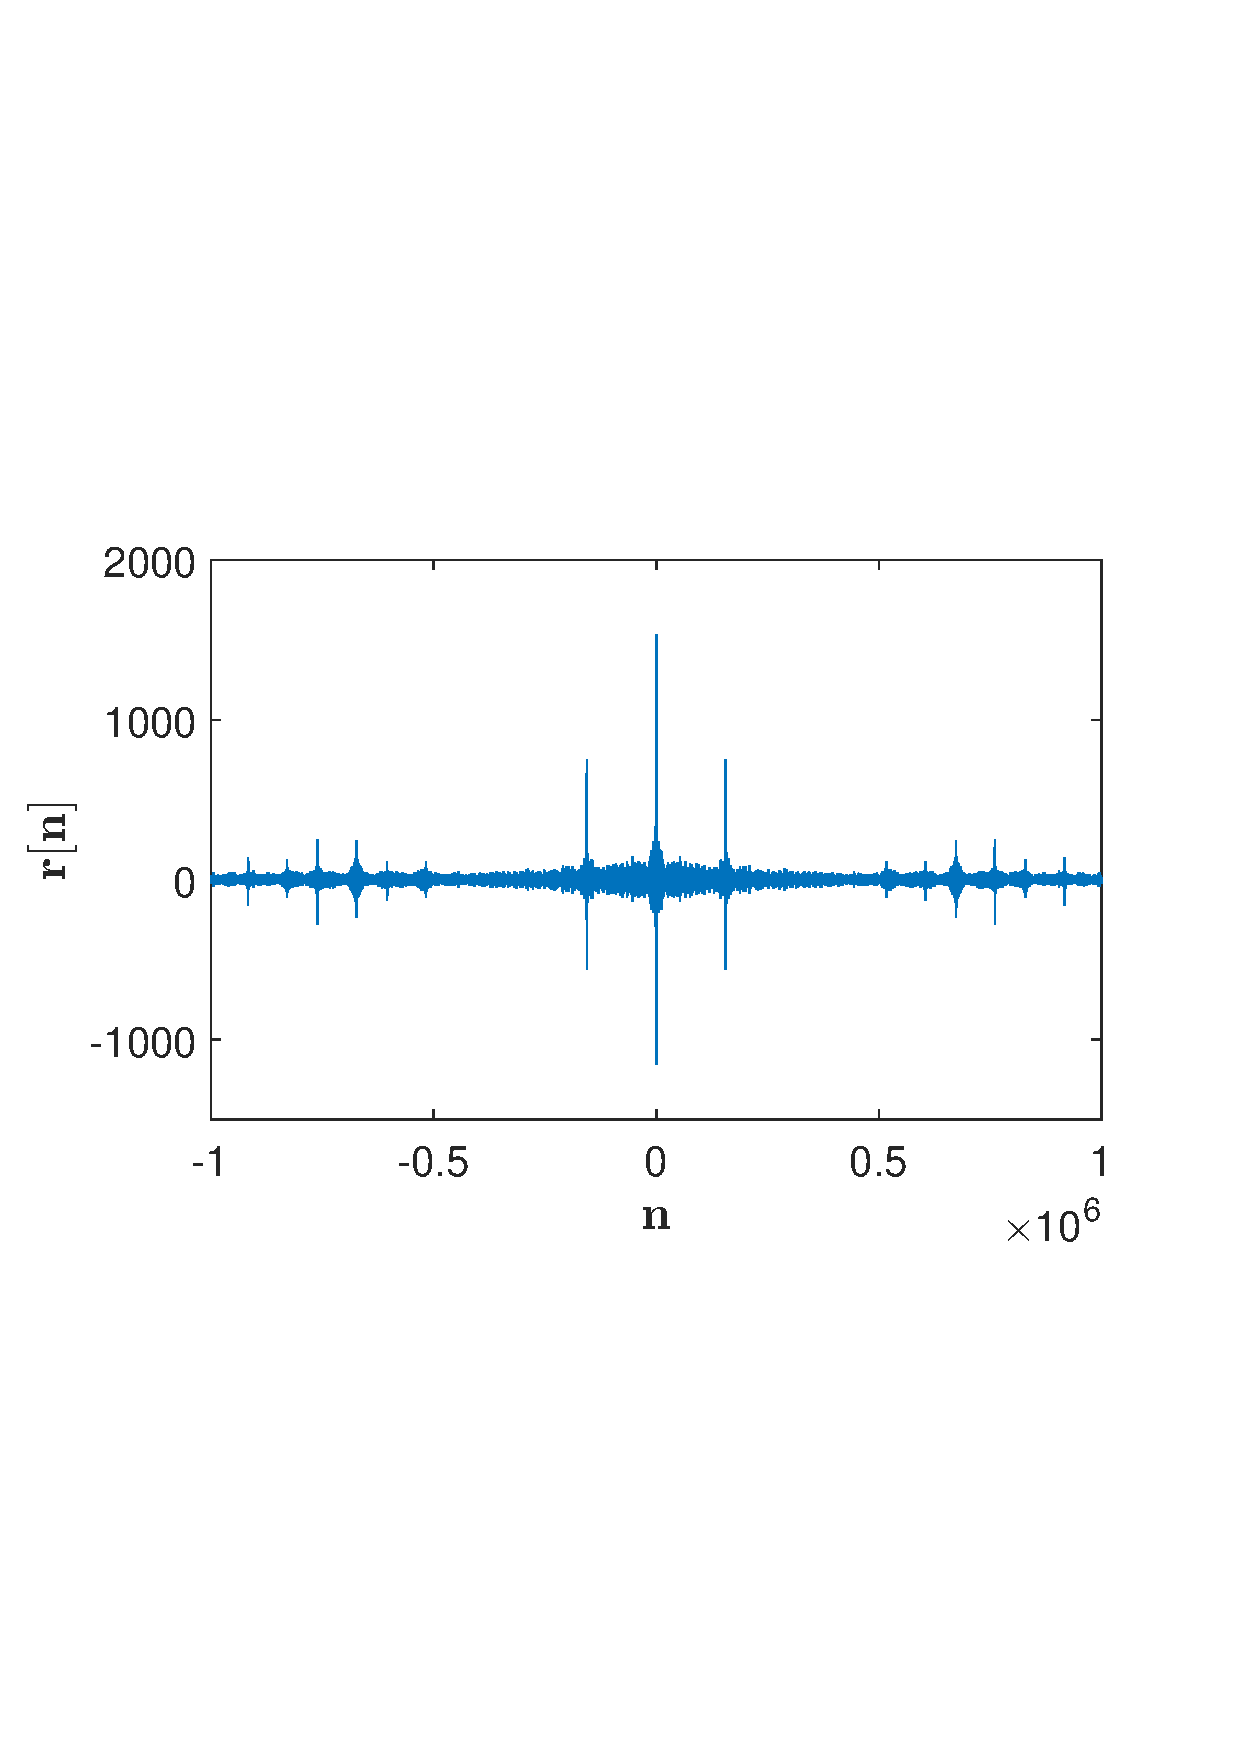
\includegraphics[trim = 0 50mm 0 80mm, clip, width=\linewidth]{fig1.pdf}
    \caption{
        Korrelationen $r[n]$ 
        \label{fig:z}
    }
\end{figure}

Korrelationen av \yhat  plottades, se figur \ref{fig:z}, och utifrån denna beräknades $\tau_2 - \tau_1$ genom att först beräkna $n_\Delta$, antalet sampel mellan
den mittersta och den högra av ovannämnda pikar. Detta räknades sedan om till en tidsdifferens genom att multiplicera resultatet
sampeltiden.

Tidsdifferensen användes sedan för att filtrera ut ekot. Detta gjordes i tidsdomänen genom att gå igenom varje sampelvärde
från $n_\Delta$ till det sista, och för varje sampelvärde, $n_i$ sätta 
\begin{equation}
x[n_i] \coloneqq x[n_i] - 0,9x[n_i - n_\Delta] 
\label{e4}
\end{equation}
där $x[n] \coloneqq \hat{y}[n]$ från början.

Operationen (\ref{e4}) fungerar, eftersom att (om man bortser från noll-värden i början av signalen som ej påverkar resultatet) ekot börjar $n_\Delta$
sampel efter själva signalen; det finns alltså ett fönster av $n_\Delta$ sampel i början av signalen som saknar eko. Genom att
värden från detta fönster subtraheras från värden $n_\Delta$ samples senare, kancelleras ekot. Eftersom att man tilldelar $x$ det ekofria
värdet samtidigt som det används i uträkningen, flyttar man detta fönster framför sig tills man nått slutet av signalen.

\subsection{Bestämning av $f_c$}

\begin{figure}[h]
    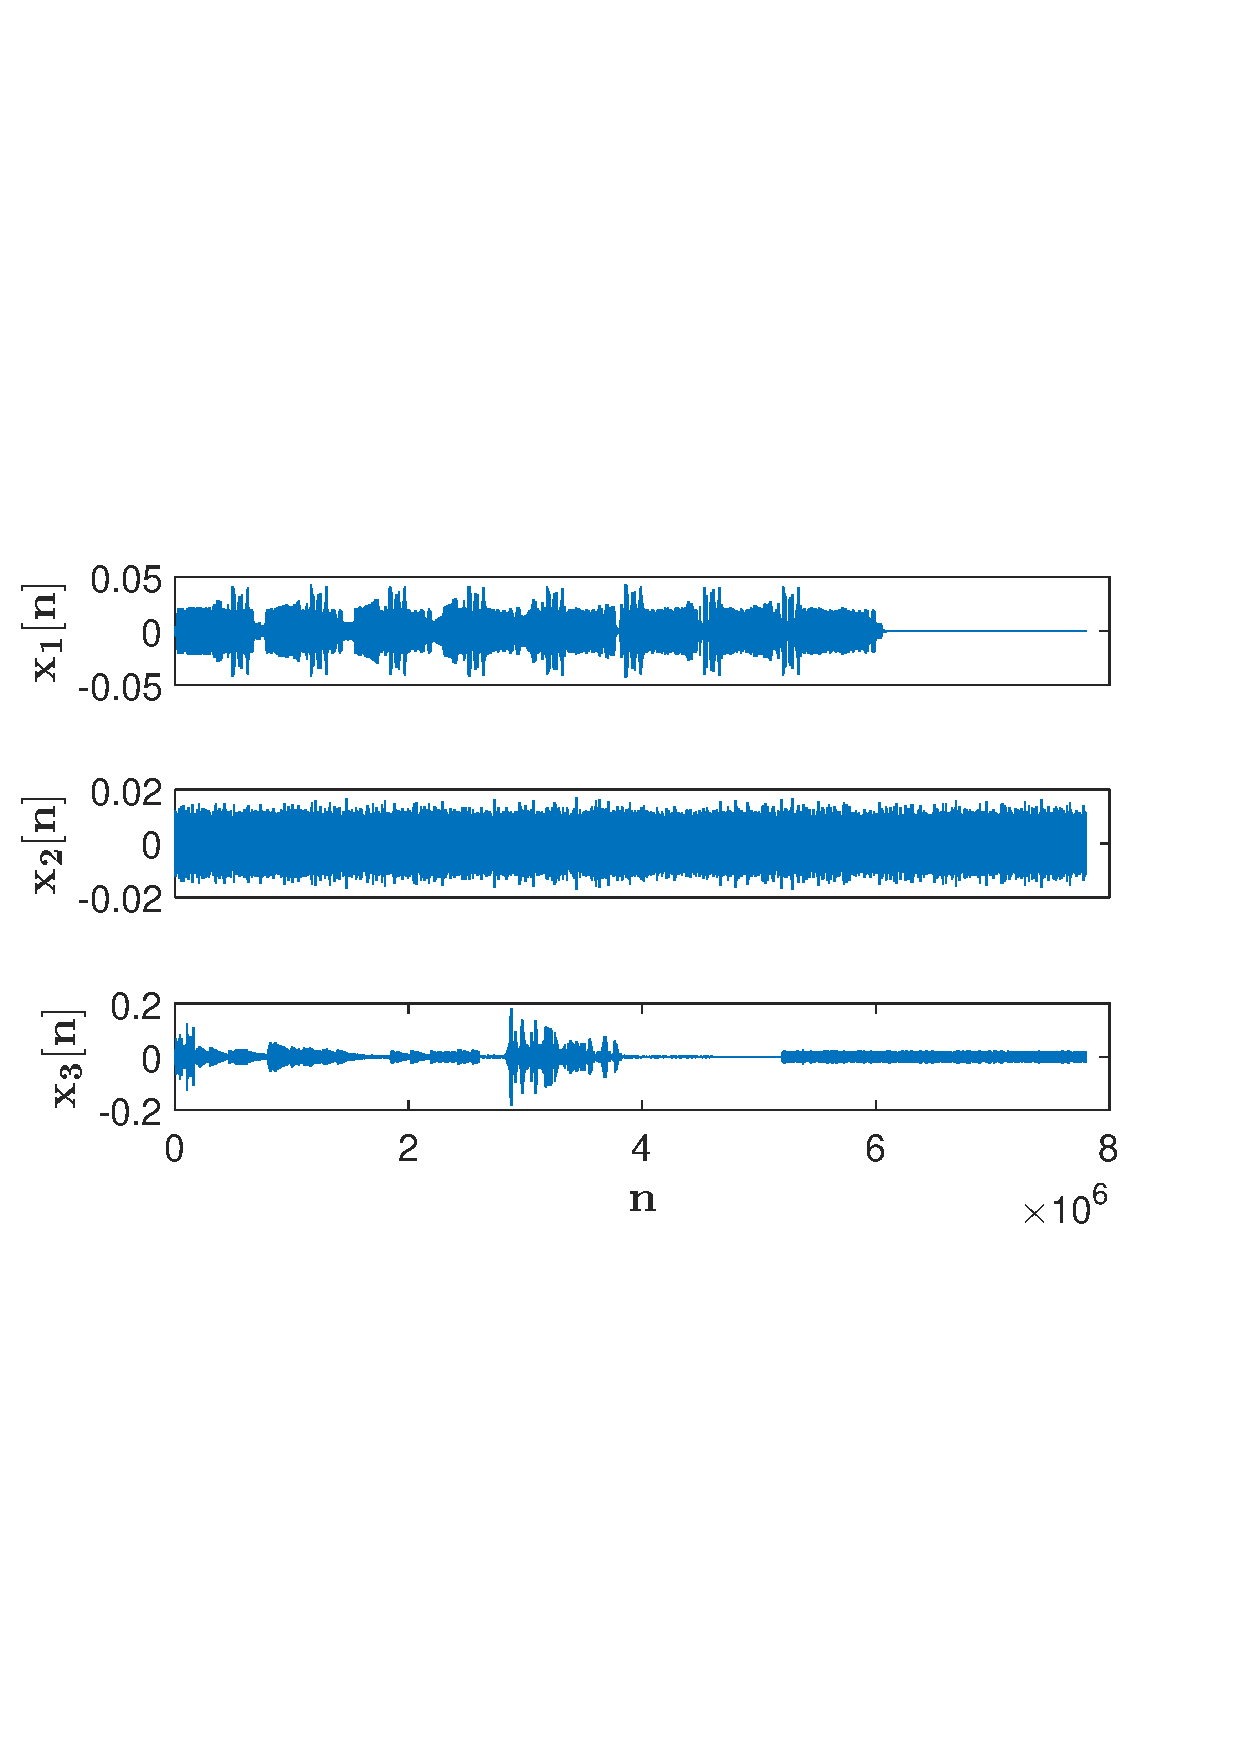
\includegraphics[trim = 0 50mm 0 80mm, clip, width=\linewidth]{fig2.pdf}
    \caption{
        den sökta signalen $x_t[n]$ 
        \label{fig:xt}
    }
\end{figure}

Genom att plotta $Y[F]$, den diskreta fouriertransformen av \yhat, kunde tre tydliga frekvensband med
centra kring sampelnummer, som motsvarade multiplar av 19 kHz, observeras.
Dessa undersöktes var för sig i tidsdomänen, för att hitta nyttosignalen $x_t[n]$ (dvs $x[n] - z[n]$).
Undersökningen bestod i att bandpassfiltrera relevant band och inverstransformera. Ett av
dessa band hade ett utseende i tidsdomänen, som stämde väl överens med det som gavs i uppgiften; den
hade tre distinkta områden, där det sista området påminnde om vitt brus, se figur \ref{fig:xt}.
Frekvensvärdet i centrum för frekvensbandet hos detta område noterades, och antogs vara $f_c$.

\subsection{Identifiering av ordspråken}

För att identifiera ordspråket genomfördes en I/Q-demodulering av $x[n]$, enligt:
\begin{multline}
    x_i[n] = \mathcal{H}_{B/2}^{LP} \{ 2 x[n] \cos[2 \pi f_c n] \} \\
    x_q[n] = \mathcal{H}_{B/2}^{LP} \{ -2 x[n] \sin[2 \pi f_c n] \}
    \label{e5}
\end{multline}
där $B$ valdes till ett värde som var tillräckligt stort för att rymma en majoritet
av signalenergin.

Det uppstod dock ett problem i och med att $x[n]$ innehöll en tidsförskjutning $n_{\tau_1}$,
vilket medförde att de komponenter man fick ut från (\ref{e5}) innehöll
linjärkombinationer av $x_i[n]$ och $x_q[n]$. Detta kan inses genom att sätta $n := n - n_{\tau_1}$
i (\ref{e5}) och använda subtraktionsatsen för sinus och cosinus.

Eftersom att det inte fanns något enkelt sätt att bestämma $n_{\tau_1}$, togs denna fram genom
att experimentera med olika värden mellan $0$ och $2 \pi$. Efter att några värden provats
kunde man dra slutsatsen att en av melodierna var kortare en den andra och följdes av några
sekunders tystnad. Värdet på $n_{\tau_1}$ finjusterades därför tills överhörningen från den
andra signalen var minimal under denna period av tystnad.

Sist av allt nedsamplades $x_i$ respektive $x_q$ med en faktor 10 och spelades upp varpå
ordspråken kunde höras.
\section{Resultat}

Laborationen gav följande resultat:
\begin{enumerate}
\item Bärfrekvensen $f_c$ var 152 KHz. 
\item Tidsdifferensen $\tau_2 - \tau_1$ var 0.39 s.
\item Ordspråken löd dels "inget ont som inte har något gott med sig", dels "väck inte den björn som sover".
\end{enumerate}

\clearpage

\section*{Min Matlab-kod:}
\begin{spverbatim}
%%Initialize
N = 7.8*10^6;
[y,Fs] = wavread('signal-herlu184.wav');
f = Fs*linspace(0,1/2,N/2);
t = 0:1/Fs:(N-1)*1/Fs;

%% 
% Determine the tau2-tau1 by studying the 
% correlation of y with itself. The Peak
% values are derived from the plot in 
% this section
% 
y_c = xcorr(y, y);
plot(y_c);

lpeak = 7.644*10^6;
mpeak = 7.800*10^6;
rpeak = 7.956*10^6;

%tau2 - tau1 in # of samples
n_delta = rpeak-mpeak;
tau_diff = n_delta*1/Fs;

%%
% Filter out echo in the time domain.
% x is the signal with the echo removed
%
x = y;
for i = n_delta+1:length(x)
    x(i) = x(i) - 0.9*x(i-n_delta);
end

x_c1 = xcorr(x, x);
%The correlation shows that the left and
%right peaks have been removed
plot(x_c1)

%%
% Determine fc
X = fft(x);
%The plot shows three distinct bands at
%frequencies with multiples of 19 kHz
plot(f, abs(X(1:end/2)))

%Filtering out each band and inverse
%transforming it shows that the
%heighest band matches the signal
%description (three distinctive parts,
%the last one being white noise)
ze = zeros(1, N);
X_target1 = ze;
X_target2 = ze;
X_target3 = ze;
X_target1(0.2/2*N/2:0.6/2*N/2) = X(0.2/2*N/2:0.6/2*N/2);
X_target2(0.7/2*N/2:1.1/2*N/2) = X(0.7/2*N/2:1.1/2*N/2);
X_target3(1.3/2*N/2:1.7/2*N/2) = X(1.3/2*N/2:1.7/2*N/2);
X_target = X_target3;
x_target = ifft(X_target, 'symmetric');

plot(x_target)

%fc i determined by looking at the 
%centrum of the heighest band of X
fc = 152*10^3;

%% 
% Demodulate
%
% The delay of x(t) results in a phase
% shift in the xi, and xq components.
% This value lies somewhere between
% zero and pi/2. The phase shift below
% was derived by testing different 
% values until the message could be heard.
%
phase_shift = 0.8;
xi_mixer = cos(2*pi*fc*t+phase_shift);
xq_mixer = sin(2*pi*fc*t+phase_shift);
xi_ = 2*xi_mixer.*x_target;
xq_ = -2*xq_mixer.*x_target;
Xi_ = fft( xi_ );
Xq_ = fft( xq_ );

%lowpass filter
Xi = zeros(1,N);
Xq = zeros(1,N);
Xi(1:0.4/2*N/2) = Xi_(1:0.4/2*N/2);
Xq(1:0.4/2*N/2) = Xq_(1:0.4/2*N/2);
xi = ifft(Xi, 'symmetric');
xq = ifft(Xq, 'symmetric');

plot(f, abs(Xq(1:end/2)));

Fs_ = Fs/10

soundsc(xi(1:20:end), Fs/20)
pause
soundsc(xq(1:20:end), Fs/20)  

%Xi "Inget ont som inte har något gott med
%sig."
%Xq "Väck inte den björn som sover."
\end{spverbatim}

\end{document}
